\section{Rubin Observatory Commissioning}
\label{sec:commissioning}

\subsection{Commissioning Schedule}
\label{ssec:commissioning-schedule}

Figure~\ref{fig:commissioning-es-schedule} shows the detailed schedule of commissioning and early science activities relative to System First Light, as of \currentdate.
ComCam First Photon was successfully achieved on 24 October 2024.
Rubin (LSSTCam) First Photon, is currently expected on 15 April 2025 and System First Light in  July 2025 (\S~\ref{sec:timeline}). 

\begin{figure}[htb]
\centering
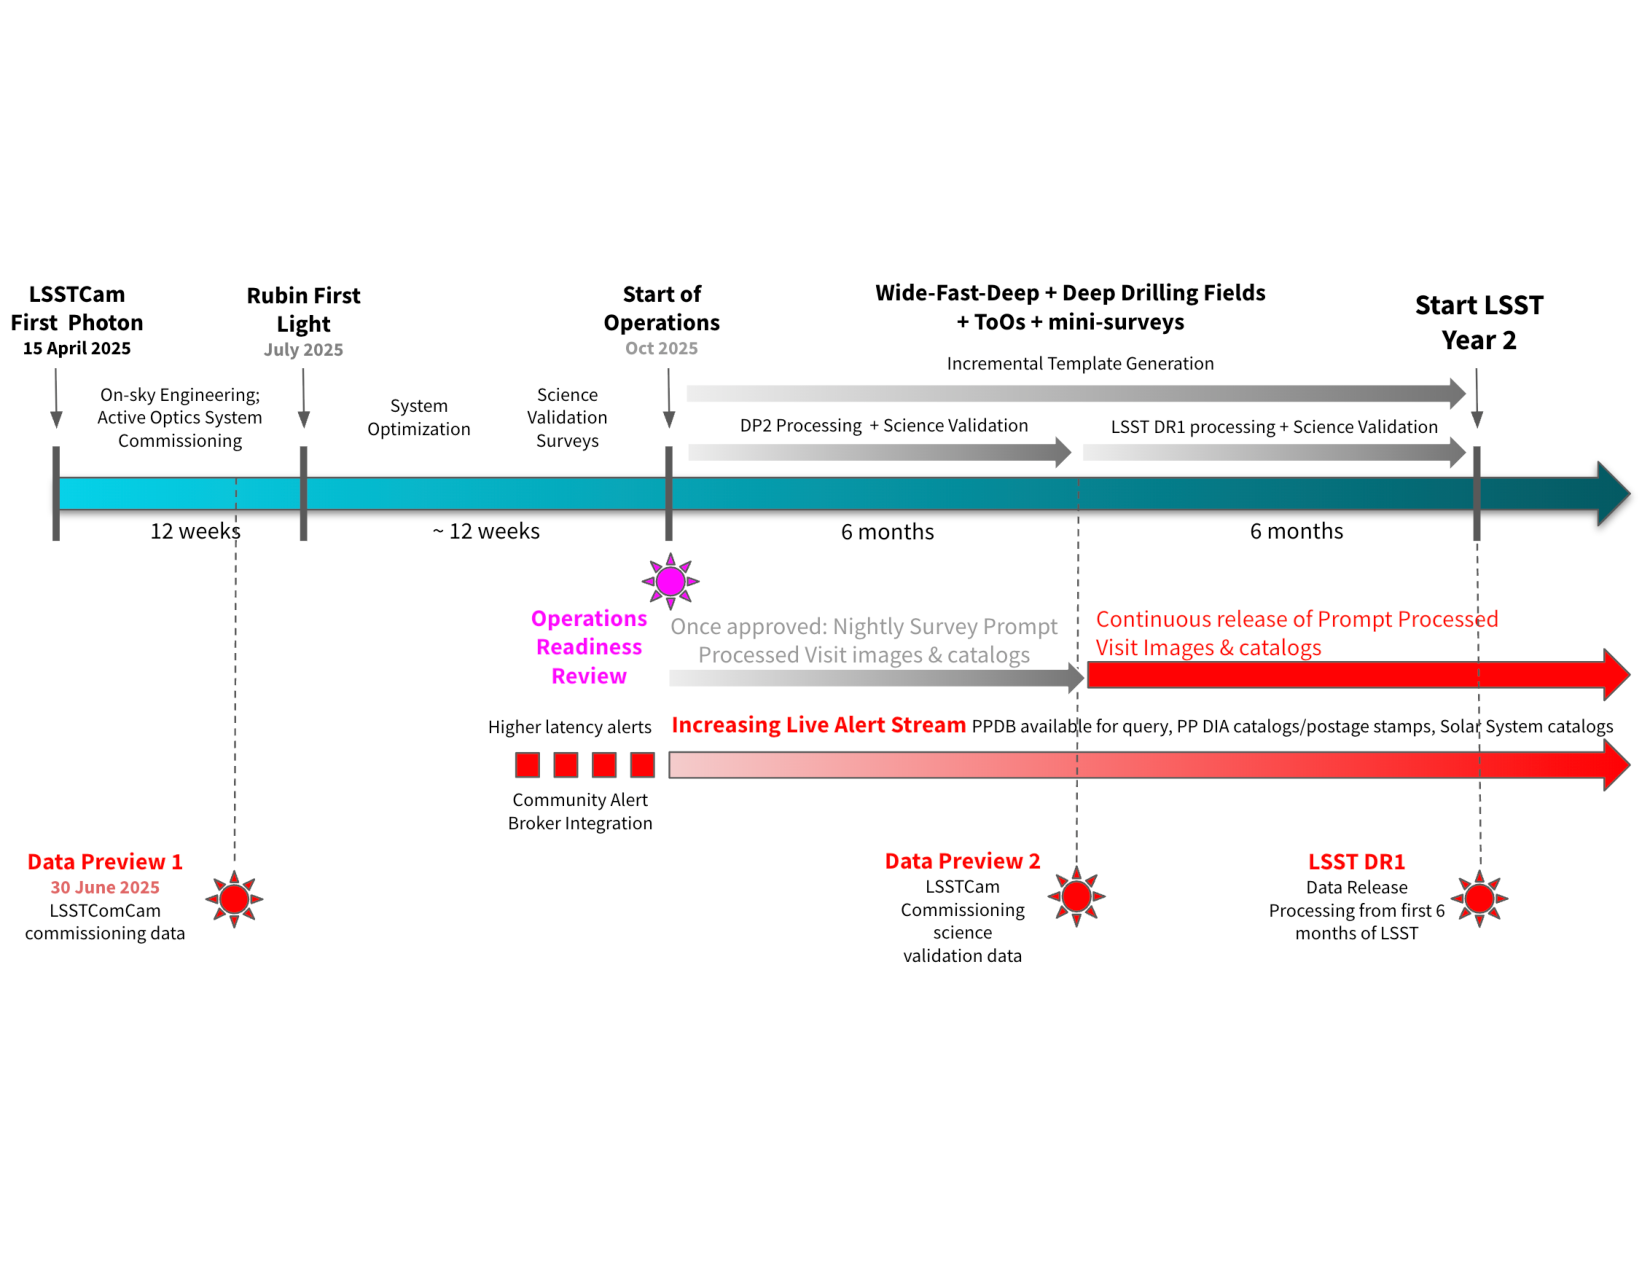
\includegraphics[width=0.98\linewidth]{figures/rubinobs_on-sky_commissioning_and_early_science.pdf}
\caption{Detailed schedule of commissioning  and early science activities relative to System First Light, as of \currentdate.}
\label{fig:commissioning-es-schedule}
\vspace{0.1cm}
\end{figure}

Rubin Observatory carried out an on-sky commissioning campaign with ComCam from 24 October 2024  through 12 December 2024, for a total of 7 weeks.
The campaign was very successful, accomplishing many goals including the optical alignment of the telescope and the delivery of science-grade images.
The median delivered image quality  for commanded in-focus images collected during the campaign, quantified in terms of the PSF FWHM, was $\approx$1.1 arcseconds. 
The best images have delivered PSF FWHM of $\approx$0.7 arcseconds.
A full report on the ComCam on-sky commissioning campaign is available at \citeds{sitcomtn-149}.

LSSTCam on-sky commissioning is currently expected to start in April 2024. (11 weeks according to the dates ... 7 weeks in the schedule)
The 8 weeks system optimization and 8 weeks SV surveys (in ops)
 
LSST data taking is expected to start before the end of 2026.
The project schedule will continue to evolve as the remaining subcomponents are delivered. 


\subsection{Commissioning Milestones}
\label{ssec:commissioning-milestones}

Commissioning work is being planned around three major milestones, \textit{ComCam First Photon}, \textit{LSSTCam First Photon} and \textit{System First Light}. 

\textbf{ComCam First Photon}: The first image of the night sky produced by photons passing through the Rubin optical system and detected by the Commissioning Camera (ComCam). 
This milestone was achieved on 24 October 2024. 

\textbf {LSSTCam First Photon}: The first image of the night sky produced by photons passing through the Rubin optical system and detected by the LSST Science Camera (LSSTCam).
Currently expected in April 2025.

\textbf {System First Light}: Defined as the point at which we can routinely acquire science-grade imaging across the LSSTCam full focal plane and have a well understood technical path towards meeting the Construction Completeness criteria   \citeds{sitcomtn-061}.
Currently expected for 4 July 2025. 

LSSTCam First Photon occurs following the successful completion of system integration. 
There are no quality criteria applied to achieving  neither the ComCam nor LSSTCam First Photon milestones. 
System First Light  marks the end of the  on-sky engineering phase and the start of the System Optimization and Science Validation phases of commissioning.
The period between ComCam First Photon and System First Light will focus on fine tuning the system including optical alignment and improving the image quality, collecting calibration data, and carrying out \textit{First Look} science programs. 

For a detailed description of all the commissioning milestones and the most current dates, see \citeds{dmtn-232}.


\subsection{Commissioning Observations}
\label{ssec:commissioning-observations}

Figure~\ref{fig:commissioning} shows the high level plan for the Rubin commissioning observations. 
Commissioning data collection is planned to take place in phases.
The \textit{On-Sky Engineering} phase may be carried out with either ComCam and/or LSSTCam, depending on future re-optimization of the sequence of integration activities (\S~\ref{ssec:commissioning-schedule})
During the \textit{System Optimization} phase,  a set of observations designed to help optimize the system will be taken during the System Optimization phase before the Science Validation Surveys are carried out. 
The SV Surveys are designed to support scientific analyses tha	t validate the system's performance, and allow Rubin to demonstrate operations readiness \citeds{SITCOMTN-005}.

\begin{figure}[htb]
\centering
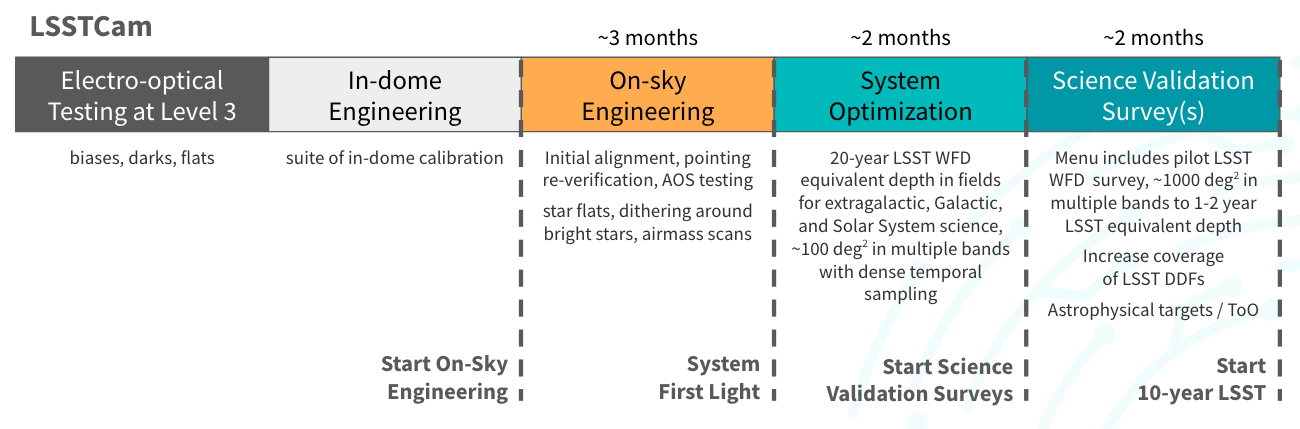
\includegraphics[width=0.95\linewidth]{figures/commissioning-plan}
\caption{Outline plan for the collection of commissioning data, as of \currentdate.}
\label{fig:commissioning}
\end{figure}

Figure~\ref{fig:commissioning} also indicates a number of planned key components of the System Optimization and SV phases.
These include a LSST wide-fast-deep (WFD) 1-2 year equivalent depth ``pilot'' survey.
Field selection will be carried out by the Commissioning Team, taking into account a wide variety of constraints as well as a ``menu'' of science opportunities to which the LSST Science Community has contributed.
Details of the plans for commissioning observations will be made available as those plans converge, in this technote and other documents as cited.